% FIXED
\section{Evaluation}
\label{s:eval}

In this section, we evaluate our AAD (not AAS) construction's proof sizes, append times and memory usage.
We find that append times and memory usage are too high for a practical deployment and discuss how they might be improved in future work (see \cref{s:eval:append-time,s:eval:memory}).
If they are improved, we find AADs can save bandwidth relative to CT and CONIKS and we describe exactly when and how much in ~\cref{s:eval:worth-it}.

\parhead{Codebase and testbed.}
We implemented our \textit{amortized} AAD construction from \cref{s:aad} in 5700 lines of C++.
Its \textit{worst-case} append time is $O(\lambda n \log^2{n})$ while its amortized append time is $O(\lambda \log^3{n})$.
We used Zcash's \texttt{libff}~\cite{libff} as our elliptic curve library with support for a 254-bit Barretto-Naehrig curve with a Type~III pairing~\cite{bn-curve}.
% 110 bits for BN254: https://eprint.iacr.org/2016/1102.pdf
We used \texttt{libfqfft}~\cite{libfqfft} to multiply polynomials and \texttt{libntl}~\cite{libntl} to divide polynomials and compute GCDs.
Our code is available at:
\begin{center}
    \url{https://github.com/alinush/libaad-ccs2019}.
\end{center}
We ran our evaluation in the cloud on Amazon Web Services (AWS) on a r4.16xlarge instance type with 488 GiB of RAM and 64 VCPUs, running Ubuntu 16.04.4 (64-bit).
This instance type is ``memory-optimized'' which, according to AWS, means it is ``designed to deliver fast performance for workloads that process large data sets in memory.''

\begin{figure*}
\centering
\subfloat[Lookup proof (worst-case AAD sizes)]{\label{f:lookup-worst}%
    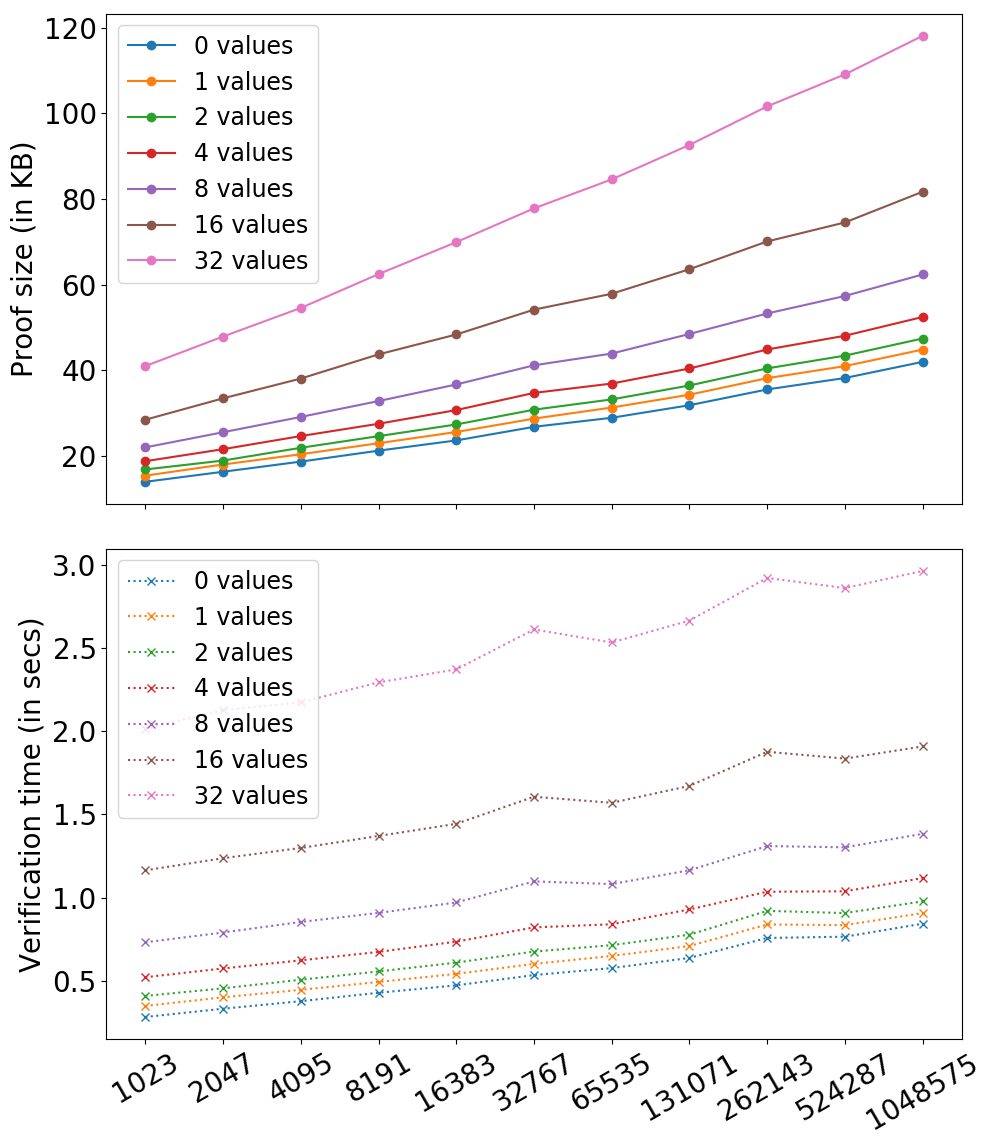
\includegraphics[width=0.32\linewidth]{figures/aad-memb-worst-case.png}
    \label{f:evaluation:lookup-worst}
}
\subfloat[Lookup proof (average-case AAD sizes)]{\label{f:lookup-avg}%
    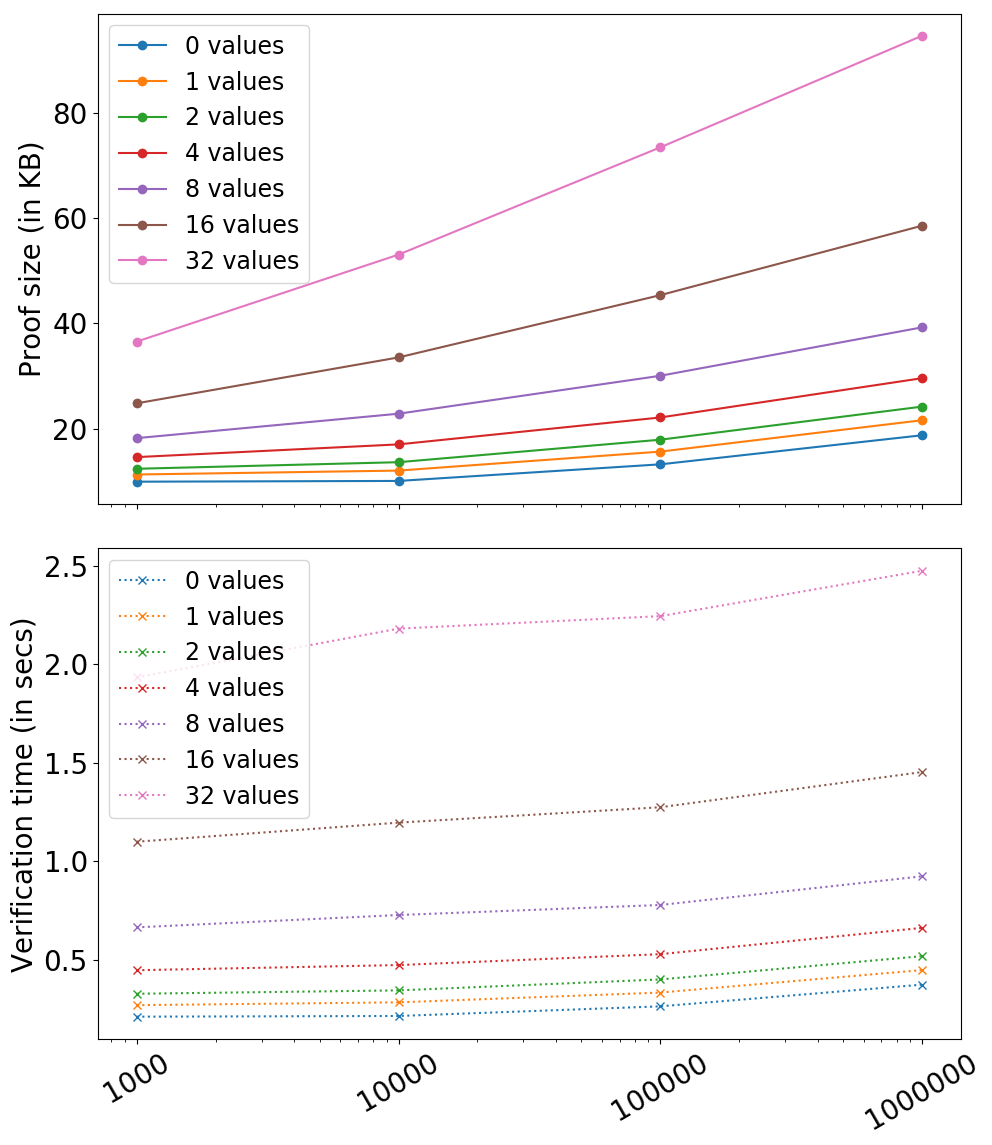
\includegraphics[width=0.32\linewidth]{figures/aad-memb-avg-case.png}
    \label{f:evaluation:lookup-avg}
}
\subfloat[Append times ($\uparrow$) and append-only proofs ($\downarrow$)]{\label{f:append-time}\label{f:append-only-proof}%
    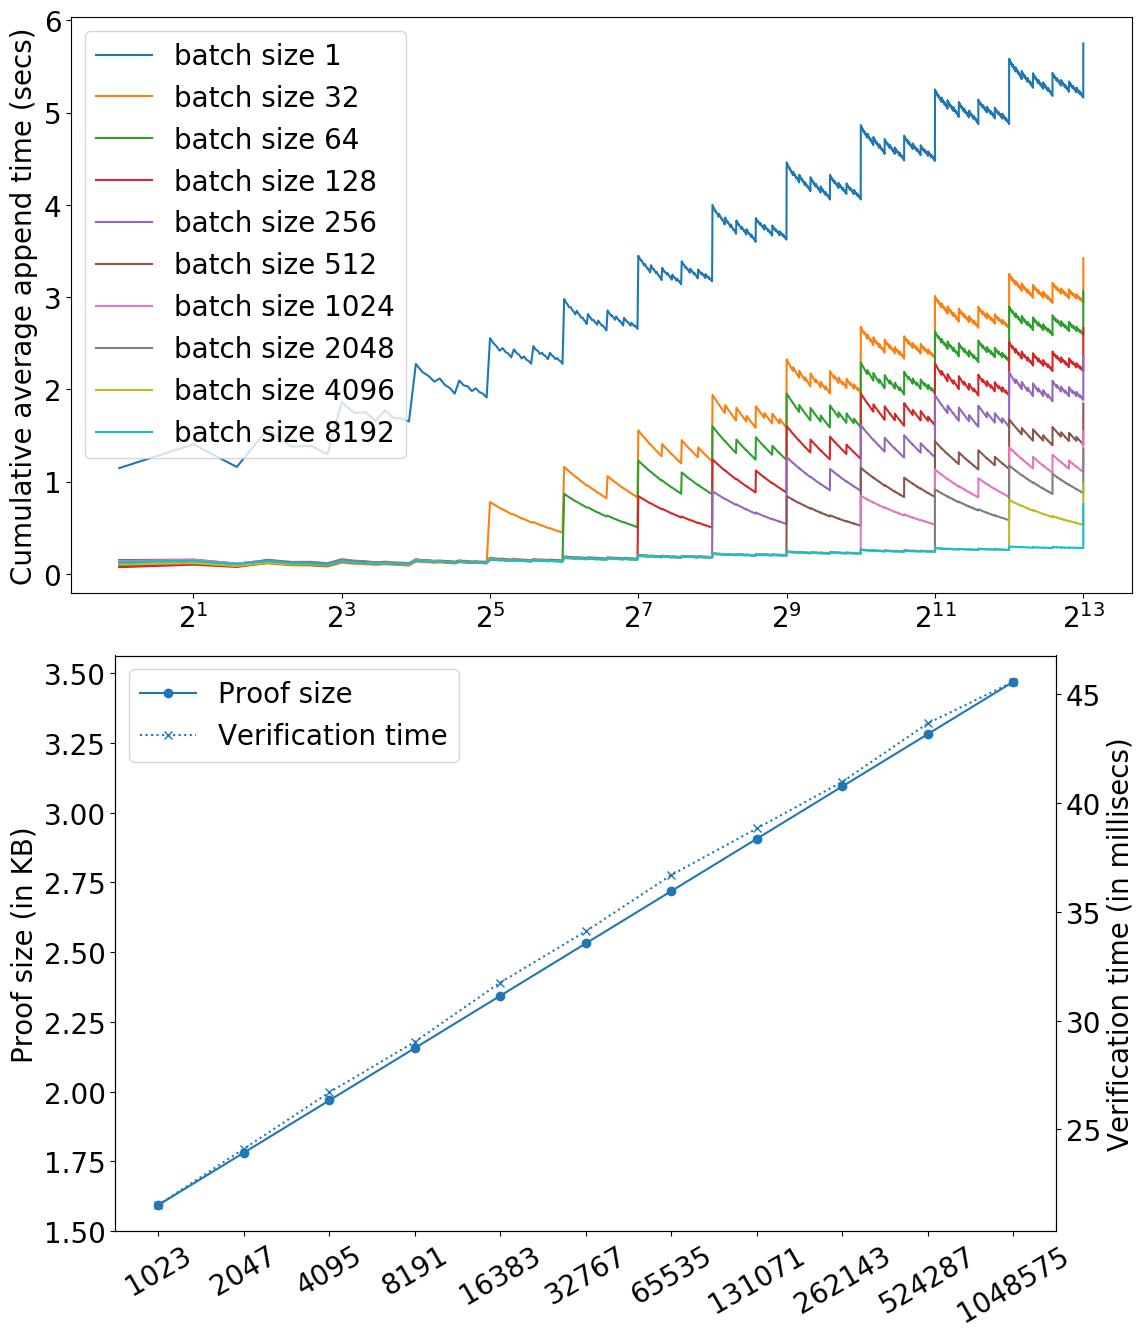
\includegraphics[width=0.32\linewidth]{figures/aad-merged-append-time-and-proof.png}
    \label{f:evaluation:append-time-and-proof}
}
\caption{
The x-axes always indicate AAD sizes.
\cref{s:eval:lookup,s:eval:append-only-proof,s:eval:append-time} explain the experiments.
In \cref{f:evaluation:append-time-and-proof} ($\uparrow$), ``spikes'' occur when two trees of size $B$ are merged, which triggers a new BFT computation, where $B$ is the batch size.
}
\label{f:evaluation}
\end{figure*}

\subsection{Microbenchmarks}

\subsubsection{Append times}
\label{s:eval:append-time}
% batch size 32
% 2019-02-04 10:50:34 36714 36714  PERF         benchAppends: 196 | Average time per append: 3422 milliseconds
% 
% batch size 64
% 2019-02-04 02:54:48 35509 35509  PERF         benchAppends: 196 | Average time per append: 3064 milliseconds
%
% batch size 128
% 2019-02-03 19:48:54 34590 34590  PERF         benchAppends: 196 | Average time per append: 2664 milliseconds
%
% batch size 256
% 2019-02-03 13:38:04 34156 34156  PERF         benchAppends: 196 | Average time per append: 2361 milliseconds
%
% batch size 512
% 2019-02-03 08:08:40 33620 33620  PERF         benchAppends: 196 | Average time per append: 1848 milliseconds
%
% batch size 1024
% 2019-02-03 03:13:40 30937 30937  PERF         benchAppends: 194 | Average time per append: 1548 milliseconds
%
% batch size 2048
% 2019-02-02 23:30:41 30167 30167  PERF         benchAppends: 194 | Average time per append: 1353 milliseconds
%
% batch size 4096
% 2019-02-02 20:15:01 29514 29514  PERF         benchAppends: 194 | Average time per append: 976 milliseconds
%
% batch size 8192
% 2019-02-02 17:47:11 28621 28621  PERF         benchAppends: 194 | Average time per append: 760 milliseconds
%

Starting with an empty AAD, we append key-value pairs to it and keep track of the \textit{cumulative average append-time}.
Recall that appends are amortized in our construction (but can be de-amortized using known techniques~\cite{overmars-van-leeuwen,overmars}).
As a result, in our benchmark some appends are very fast (e.g., 25 milliseconds) while others are painfully slow (e.g., 1.5 hours).
To keep the running time of our benchmark reasonable, we only benchmarked $2^{13} = 8192$ appends.
We also investigate the effect of batching on append times.
Batching $k = 2^i$ appends together means we only compute one BFT for the full tree of size $k$ created after inserting the batch.
In contrast, without batching, we would compute $k$ BFTs, one for each new forest root created after an append.
\cref{f:append-time} shows that the average append time is 5.75 seconds with no batching and 0.76 seconds with batch size 8192.
(For batch sizes $32, 64, \dots, 4096$, the average times per append in milliseconds are 3422, 3064, 2644, 2361, 1848, 1548, 1353 and 976 respectively.)
These times should increase by around 3.5 seconds if we benchmarked $2^{20}$ appends.

\parhead{Speeding up appends.}
The bottleneck for appends is computing the BFTs.
Although we used \texttt{libff}'s multi-threaded multi-exponentiation to compute accumulators faster, there are other ways to speed up appends that we have not explored.
First, we can parallelize computing (1) the polynomials on the same level in a BFT, (2) the smaller accumulators at lower levels of the BFT, where multi-threaded multi-exponentiation does not help as much and (3) the subset proofs in the forest.
Second, we can reuse some of the previously computed accumulators when computing a new BFT.
Third, our BPT and BFT constructions require ``extractable'' counterparts of the accumulators, which almost triple the time to commit to a polynomial.
We hope to remove this expensive requirement by proving our construction secure in the generic group model, similar to new SNARK constructions~\cite{groth16}.
Finally, techniques for distributed FFT could speed up polynomial operations~\cite{dizk}.

\subsubsection{Lookup proofs}
\label{s:eval:lookup}
We investigate three factors that affect lookup proof size and verification time: (1) the dictionary size, (2) the number of trees in the forest and (3) the number of values of a key.
Our benchmark creates AADs of ever-increasing size $n$.
For speed, instead of computing accumulators, we simply pick them uniformly at random.
(Note that this does not affect the proof verification time.)
We measure \textit{average} proof sizes for keys with $\ell$ values in an AAD of size $n$, where $\ell \in \{0, 1, 2, 4, 8, 16, 32\}$.
(Recall that a key with $\ell$ values requires $\ell$ frontier proofs.)
To get an average, for every $\ell$, we set up 10 different \textit{target} keys so each key has $\ell$ values.
The rest of the inserted keys are random (and simply ignored by the benchmark).
Importantly, we randomly disperse the target key-value pairs throughout the forest to avoid having all values of a key end up in consecutive forest leaves, which would artificially decrease the proof size.
Once the dictionary reaches size $n$, we go through every target key with $\ell$ values, compute its lookup proof, and measure the size and verification time.
% (Think of a lookup proof for $\ell = 0$ values as a non-membership proof.)
Then, for each $\ell$, we take an average over its 10 target keys.
We repeat the experiment for increasing dictionary sizes $n$ and summarize the numbers in \cref{f:lookup-avg,f:lookup-worst}.
Proof verification is single-threaded.

\parhead{Worst-case versus best-case dictionary sizes.}
Recall that some dictionary sizes are ``better'' than others because they have fewer trees in the forest.
For example, a dictionary of (worst-case) size $2^i - 1$ will have $i$ trees in the forest and thus $i$ BFTs.
Thus, a lookup proof must include frontier proofs in all $i$ BFTs.
In contrast, a dictionary of size $2^i$ only has a single tree in the forest, so a lookup proof needs only one {frontier proof}.
Indeed, our evaluation shows that lookup proofs are smaller in AADs of size $10^i$ (see \cref{f:lookup-avg}) compared to $2^i-1$ (see \cref{f:lookup-worst}).
For example, for a key with 32 values, the proof averages 95 KiB for size $10^6$ and 118 KiB for size $2^{20} - 1$.

%  aadSize  numValues  proofKiB    verifSecond
%  1000000          0   18.718750    0.372885
%  1000000          1   21.578125    0.446906
%  1000000          2   24.168750    0.517544
%  1000000          4   29.578125    0.661258
%  1000000          8   39.250000    0.923060
%  1000000         16   58.587500    1.452599
%  1000000         32   94.728125    2.474843

%  aadSize  numValues  proofKiB    verifSecond
%  1048575          0   41.934375    0.843512
%  1048575          1   44.803125    0.907273
%  1048575          2   47.390625    0.977507
%  1048575          4   52.418750    1.117400
%  1048575          8   62.350000    1.383276
%  1048575         16   81.684375    1.908019
%  1048575         32  118.112500    2.962104

\subsubsection{Append-only proofs}
\label{s:eval:append-only-proof}
This benchmark appends random key-value pairs until it reaches a target size $n = 2^{i+1} - 1$.
Then, it measures the append-only proof size (and verification time) between AADs of size $n$ and $m = 2^{i} - 1$.
We benchmarked on $2^{i}-1$ AAD sizes to illustrate worst-case $\Theta(i)$ append-only proof sizes.
To speed up the benchmark, we randomly pick accumulators in the forest.
Append-only proof verification is single-threaded.
Our results show append-only proofs are reasonably small and fast to verify (see \cref{f:append-only-proof}).
For example, the append-only proof between sizes $2^{19}-1$ and $2^{20}-1$ is 3.5 KiB and verifies in $45$ milliseconds.

\subsubsection{Memory usage.}
\label{s:eval:memory}
% Note: The 390x is from the FrontierSizeBench numbers in experiments/ccs19/frontier-size/20
\newcommand{\frontierOverhead}{390}
Our lookup proof benchmark was the most memory-hungry: it consumed 263 GiB of RAM for AAD size $n = 2^{20}-1$.
In contrast, the append-only proof benchmark consumed only 12.5 GiBs of memory, since it did not need BFTs.
As an example, when $n = 2^{20} - 1$, all BFTs combined have no more than $\frontierOverhead n$ nodes.
% This would normally require $2\cdot 32 + 64 = 128$ bytes per node, but \texttt{libff} needs 96 bytes per G1 and 192 per G2 => 384 for 2*G1 + G2
Since we are using Type~III pairings, each node stores three accumulators (two in $\Group_1$ and one in $\Group_2$) in 384 bytes (due to \texttt{libff}'s 3x overhead).
Thus, the BFT accumulators require no more than 147 GiB of RAM.
% 400 * (2^20-1) * (32*2 + 64) bytes in GiB        ----> 50 GiBs     (accs ideal)
% 400 * (2^20-1) * (96*2 + 192) bytes in GiB       ----> 150 GiBs    (accs w/ libff)
% 390 * (2^20-1) * (96*2 + 192) bytes in GiB       ----> 146.24 GiBs (accs w/ libff)
%
% Each node stores: left, right, parent and data pointer: 8*4 = 32 bytes
% 390 * (2^20-1) * (8*4) bytes in GiB              ----> 12.18 GiB   (root BFT pointer overhead)
% 450 * (2^20-1) * (8*3) bytes in GiB              ----> 10.54 GiB   (root BPT pointer overhead)
The rest of the overhead comes from our pointer-based BFT implementation and other bookkeeping (e.g., polynomials).
% $q$-PKE public parameters for an AAD of size $2^{20}$ take up at least 64 GiB of RAM: 512 * 2^20 * (32 bytes * 2 + 64 bytes), ignoring libff's 3x overhead.
The $q$-PKE public parameters could have added 64 GiBs of RAM, but these two benchmarks did not need them.

\parhead{Improving memory.}
A new security proof could eliminate the additional $\Group_1$ and $\Group_2$ accumulators and reduce BFT memory by 2.66x and the size of the public parameters by 1.33x (see \cref{s:eval:append-time}).
% i.e., in each pair of BFT siblings, we go from 2 * [ G_1, G_1, G_2 ] (32*2 + 64 bytes) to [ G_1 ] (32 bytes) in one node and [ G2 ] (64 bytes) in the sibling (so they can be paired)
% saves 2*(32+64) / (32 + 64) = 2.66x memory
% and eliminates g_1^{\tau s^i}'s, saving (32 * 2 + 64) / (32 + 64) = 1.33x memory
A more efficient representation of group elements than \texttt{libff}'s could also reduce BFT memory by 3x.
An efficient array-based implementation of BPTs and BFTs could further reduce memory by tens of gigabytes.
Finally, the 390x overhead of BFTs can be drastically reduced by carefully grouping upper frontier prefixes together in a BFT leaf, similar to the grouping of lower frontier prefixes from \cref{s:aad}.
However, doing this without increasing the lookup proof size too much remains to be investigated.
% The idea is that right now, each upper frontier prefix gets its own BFT leaf.
% This is because when proving non-membership of a key, we have to give a frontier proof for one of its missing prefixes.
% We do this by giving a subset path to a BFT leaf containing \textit{just} that missing prefix.
% But this means we incur a large computational overhead, creating roughly 2\lambda leaves for every newly inserted key's upper frontier prefixes.
% We could reduce this drastically by grouping upper frontier prefixes too (similar to how we group lower frontier prefixes).
% The downside is that, now, a frontier proof for an upper frontier prefix will be sending a path to a leaf with several other prefixes.
% To verify the leaf accumulator of this path, the verifier will have to recreate it from scratch.
% So he will need to be given the other/extra upper frontier prefixes in that leaf.
% This will slightly increase proof sizes, but could be mitigated against with compression.

\subsection{Comparison to Merkle tree approaches}
\label{s:eval:comparison-to-merkle}

How do AADs compare to Merkle prefix trees or History Trees (HTs), which are used in CONIKS and Certificate Transparency (CT) respectively?
First of all, appends in AADs are orders of magnitude slower because of the overheads of cryptographic accumulators and remain to be improved in future work (see \cref{s:eval:append-time}).

Lookup proofs in prefix trees are much smaller than in AADs.
% $\log_2(2^{20}) \cdot 32 = 640$ bytes
In a prefix tree of size $2^{20}$, a proof consisting of a Merkle path would be around $640$ bytes.
In comparison, our proofs for a key with 32 values are 152 times to 189 times more expensive (depending on the number of trees in the forest).
% 95 KiB / 640 bytes = 152x
% 118 KiB / 640 bytes = 189x
On the other hand, append-only proofs in AADs are $O(\log{n})$, much smaller than the $O(n)$ in prefix trees.
For example, our Golang implementation of prefix trees, shows that the append-only proof between trees of size $2^{19}$ and $2^{20}$ is 32 MiB (as opposed to 3.5 KiB in AADs).
The proof gets a bit smaller when the size gap between the dictionaries is larger but not by much: 14.6 MiB between $10^5$ and $10^6$.

Lookup proofs in history trees (HTs) are $O(n)$-sized, compared to $O(\log^2{n})$ in AADs.
This is because, to guarantee completeness, the HT proof must consist of all key-value pairs.
On the other hand, append-only proofs in AADs are slightly larger than in HTs.
While our proofs contain approximately the same number of nodes as in HT proofs, our nodes store two BPT accumulators in $\Group_1$ and a subset proof in $\Group_2$ (in addition to a Merkle hash).
This increases the per-node proof size from 32 bytes to 32 + 64 + 64 = 160 bytes.

% Sparse Merkle prefix tree proof sizes
% oldSize   newSize     appendOnlyProfSize
% 524,288   1,048,576   32 MiB
% 100,000   1,000,000   14.3 MiB

% Append-only proof sizes:
%  newDictSize  proofKiB  verifyMillisec
%         1023     1.59375      21.521
%         2047     1.78125      24.105
%         4095     1.96875      26.698
%         8191     2.15625      29.022
%        16383     2.34375      31.749
%        32767     2.53125      34.103
%        65535     2.71875      36.689
%       131071     2.90625      38.830
%       262143     3.09375      40.976
%       524287     3.28125      43.664
%      1048575     3.46875      45.573


\subsubsection{When do AADs reduce bandwidth?}
\label{s:eval:worth-it}
Asymptotically, AAD proof sizes outperform previous work.
But in practice, our evaluation shows AAD proof sizes are still larger than ideal, especially lookup proofs.
This begs the question: \textit{In what settings do AADs reduce bandwidth in transparency logs?}
We answer this question below while acknowledging that AAD append times and memory usage are not yet sufficiently fast for a practical deployment (see \cref{s:eval:append-time}).

\newcommand{\coniksfreq}{\ensuremath{\mathbf{\mathsf{D}}}\xspace}
\newcommand{\checkfreq}{\ensuremath{\mathbf{\mathsf{C}}}\xspace}

Consider a key transparency log with approximately one billion entries (i.e., an entry is a user ID and its PK).
If this were a CONIKS log, then each user must check their PK in every digest published by the log server.
Let \coniksfreq denote the number of digests published per day by the log server.
This means the CONIKS log server will, on average, send $960 \cdot \coniksfreq$ bytes per day per user (without accounting for the overhead of VRFs~\cite{vrf} in CONIKS).
If this were an AAD log, then each user (1) gets the most recent digest via an append-only proof and (2) checks their PK only in this digest via a lookup proof.
Let \checkfreq denote the number of times per day a user checks his PK (and note that, in CONIKS, $C = D$).
Since the lookup proof is for the user's PKs not having changed, it only needs to contain frontier proofs.
Extrapolating from \cref{f:lookup-avg}, such an average-case lookup proof is 40 KiB (in an AAD of size one billion).
Similarly, an append-only proof would be 7 KiB.
This means the AAD log server will, on average, send $47 \cdot 1024 \cdot C$ bytes per day per user.
Thus, AADs are more efficient when $.0199 \cdot D / C > 1$.
% Thus, if $C < (960 \cdot D) / (47\cdot 1024) =  0.0199 \cdot D$, then the AAD log server requires less bandwidth than CONIKS.
In other words, AADs will be more bandwidth-efficient in settings where log digests must be published frequently (i.e., $D$ is high) but users check their PK sporadically (i.e., $C$ is low).
% This should already be the case in key transparency, where all users should be able to register and update keys quickly (for availability reasons) even though some users might check their keys less often (since users can be offline).
For example, if $D=250$ (i.e., a new digest every 6 minutes) and $C=0.5$ (i.e., users check once every two days), then AADs result in 10x less bandwidth.

%% In CT, the server has to send   (certs_per_sec * cert_size_bytes * num_monitors)               bytes / sec
%% In AADs, the server has to send (47 * 1024 / (3600 * 24) * num_monitors * monitorings_per_day) bytes / sec
%%                                  .557 * num_monitors * monitorings_per_day)                    bytes / sec
%%
%% CT / AAD bandwidth overhead: 
%%      certs_per_sec * cert_size_bytes / (.557 * monitorings_per_day)
%%      17318 / (.557 monitorings_per_day)
%%      e.g., 1295.481 when monitoring once per hour (which is consistent with 483 GiBps / 383 MiBps)
%%
%% As long as:
%%      monitorings_per_day < certs_per_sec * cert_size_bytes / (47*1024/(3600*24))
%%      monitorings_per_day < certs_per_sec * cert_size_bytes / .557
%%      monitorings_per_day < 31,091.56
%% ...AADs result in less bandwidth.
What about CT?
Recall that CT lacks succinct lookup proofs.
As a result, domains usually trust one or more \textit{monitors} to download the log, index it and correctly answer lookup queries.
Alternatively, a domain can act as a monitor itself and keep up with every update to the log.
We call such domains \emph{monitoring domains}.
Currently, CT receives 12.37 certificates per second on average~\cite{ct-num-certs}, with a mean size of 1.4 KiB each~\cite{ct-avg-cert-size}.
Thus, a CT log server will, on average, send $12.37 \cdot 1.4 \cdot 1024 = 17,733.63$ bytes per second per monitoring domain.
In contrast, AADs require $47 \cdot 1024 \cdot C / 86,400 = .557\cdot C$ bytes per second per monitoring domain.
As before, $C$ denotes how many times per day a monitoring domain will check its PK in the log.
Thus, AADs are more efficient when $31,837 / C > 1$.
So even if domains monitor very frequently (e.g., $C = 100$), AADs are more bandwidth efficient.
However, we stress that our append times and memory usage must be reduced for a practical deployment to achieve these bandwidth savings (see \cref{s:eval:append-time,s:eval:memory}).

%% CONIKS bandwidth
%  ----------------
% Assume the CONIKS log publishes 10,000 digests per day.
% bytes_per_user = 960 bytes * 10,000 / day = 111.11 bytes/user/sec
% bytes_total = 111.11 bytes/user/sec * 1,000,000,000 = 103 GiBps
%
% If the frequency is to update the log once per hour, then CONIKS beats AADs.
% 960 bytes * 24 / day = 0.266666667 bytes/user/sec
% multiplied by 1,000,000,000 users, that's 254.31 MiBps.
% If it's once per minute, then the bandwidth would go to 253.31 MiBps * 60 = 14.9 GiBps.
% On the other hand, the proofs can be compressed using diffs, which could save a lot of traffic.

%% AAD bandwidth for CONIKS
%  ------------------------
% 47 KiB 10^9 / day = 47 KiB * 1024 bytes/KiB * 10^9 users / (24 hr/day * 60 min/hr * 60 sec/min) = 557037037 bytes/sec = 531.23 MiBps

%% CT bandwidth
%  ------------
% First CT log was launched in March 2013. Today is July 7, 2018 ([source](https://en.wikipedia.org/wiki/Certificate_Transparency#Certificate_authority_implementation))
% 1976 days between 03/01/2013 and 07/28/2018
% 2,112,278,786 certificates
% 1068966 certs/day
% 12.37 certs/second
% 1,400 bytes: the average size of a certificate
% 12.37 certs/sec * 1,400 bytes/cert = 17,318 bytes/sec
% 17,318 bytes/sec * 30 million = 519540000000 bytes/sec =  483 GiB/sec if 30 million domains monitor

%% AAD bandwidth for CT
%  --------------------
% 47 KiB * 1024 bytes/KiB * 30 million domains / hr = (47 * 1024 * 30*10^6 / 3600) / sec = 401,066,666.667 bytes/second = 383 MiBps
